\newgeometry{total={170mm, 270mm}, voffset = 0pt}
\begin{titlepage}
    \backgroundsetup{contents={
        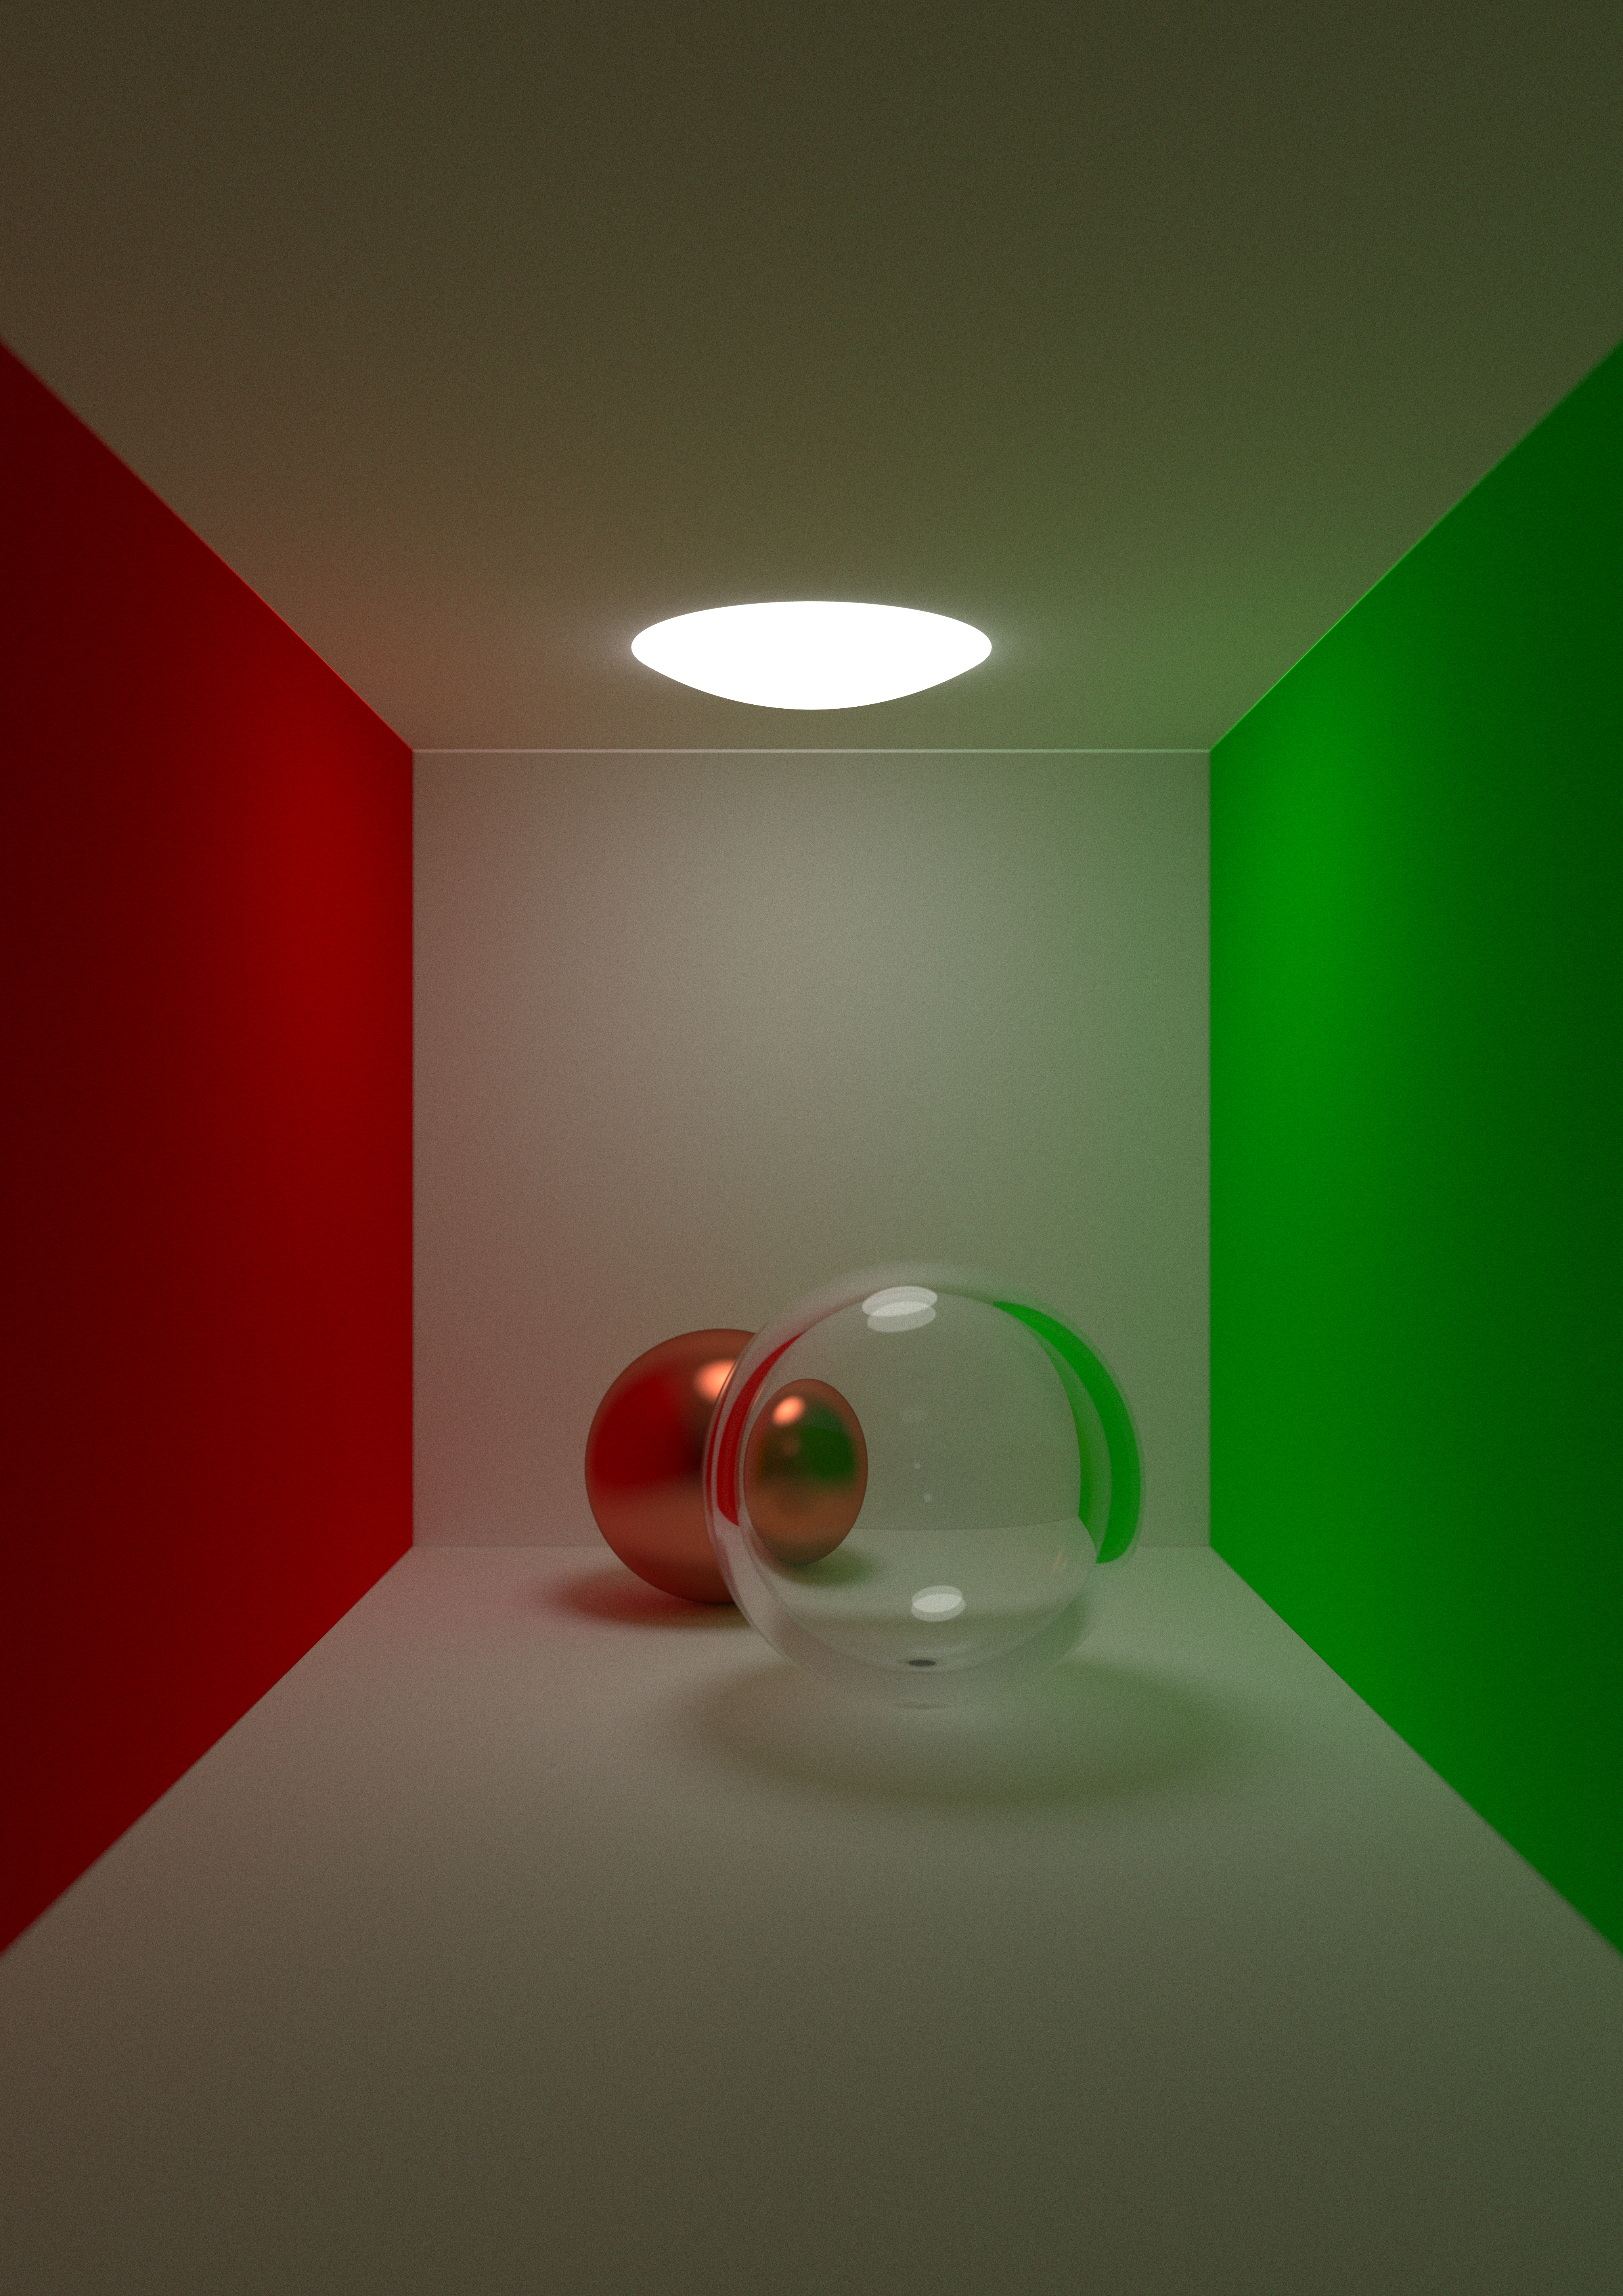
\includegraphics[]{images/title_image.png}},
        angle=0,
        scale=0.2,
        %hshift=3.5cm,
        %vshift=-0.5cm,
        opacity=1
    }
    \BgThispage
   
    \centering{
    \vspace{30cm}
    \begin{tikzpicture}[overlay] % White border around the page
        \draw[white, ultra thick]  
            (\xone mm, \yone mm)
         -- (\xtwo mm, \yone mm)
         -- (\xtwo mm, \ytwo mm) 
         -- (\xone mm, \ytwo mm)
         -- (\xone mm, \yone mm + 0.9pt); % additional length to fill the gap in the corner
    \end{tikzpicture}

    %\vspace{0.5cm}
    \color{white}
    \LARGE
    CT Projekt \\
    %\vspace{0.5cm}
    \rule{\linewidth}{1.5pt}
    \textsc{
    \Huge Raytracing \\
    }
    \vspace{-4pt}
    \rule{\linewidth}{1.5pt} \\
    %\vspace{19.7cm}
    \vspace{22cm}
    \Large
    Christian Korn

    }

\end{titlepage}
\restoregeometry